
%(BEGIN_QUESTION)
% Copyright 2006, Tony R. Kuphaldt, released under the Creative Commons Attribution License (v 1.0)
% This means you may do almost anything with this work of mine, so long as you give me proper credit

Noen elektroniske regulatorer tilbyr en {\it tidsproporsjonal} utgang i stedet for den vanlige {\it strømproporsjonale} utgangen. Med tidsproporsjonal utgang kobles regulatorens to utgangsterminaler (internt) til en relékontakt eller transistor, som bare kan slå en elektrisk last helt på eller helt av:

$$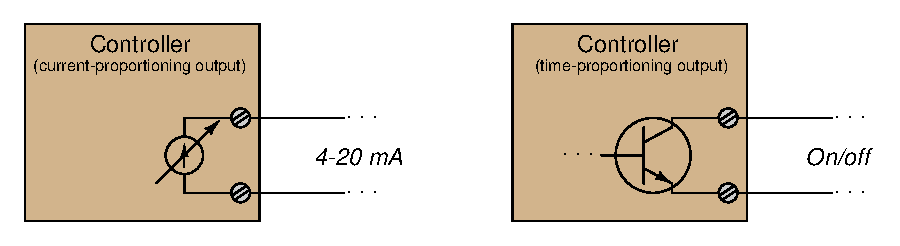
\includegraphics[width=15.5cm]{i01487x01.eps}$$

Tidsproporsjonal regulering brukes oftest når sluttelementet er en elektrisk varmer. Forklar hvordan tidsproporsjonal regulering holder en prosessvariabel på settpunkt når den bare kan slå varmeren av og på (og ikke noe mellomnivå).

\underbar{file i01487}
%(END_QUESTION)





%(BEGIN_ANSWER)

Regulatoren leverer et {\it pulsbreddemodulert} signal (PWM), der driftssyklusen i av/på-koblingen modulerer energitilførselen til prosessen gjennom varmeelementet.

%(END_ANSWER)





%(BEGIN_NOTES)


%INDEX% Control, proportional: time-proportioning output

%(END_NOTES)

